Algorytm CMA-ES to algorytm ewolucyjny, który na podstawie populacji kandydatów określa zakres wielowymiarowego rozkładu normalnego na którym generuje nowych potomków.

Jego parametry, średnia m, skala $\sigma$, oraz macierz kowariancji C — są adaptowane na podstawie wcześniej ocenionych rozwiązań

Tworzy populację kandydatów, ocenia ich jakość i na jej podstawie aktualizuje średnią i macierz kowariancji rozkładu wielowymiarowego, którą wykorzystuje do losowania nowej generacji

Przestrzeń operacji algorytmu CMAES można opisać jako $x \sim N(m, \sigma^2C)$, gdzie

$m$ - średnia rozkładu 

$\sigma$ - globalny krok

$C$ - macierz kowariancji

\begin{figure}[H]
    \centering
    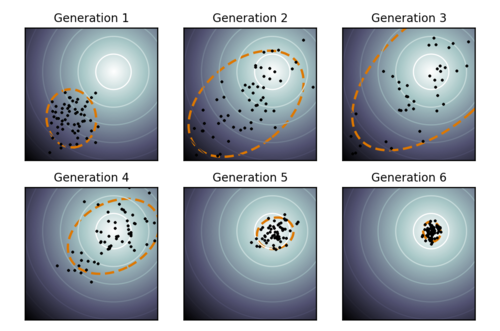
\includegraphics[width=0.7\linewidth]{algos/CMAES/range.png}
    \caption{przykładowy przebieg algorytmu w CMAES}
    % \label{fig:placeholder}
\end{figure}